\section{Architecture and Compile-Time Pipeline}

The core architecture of \texttt{ctpb} is organized as a three-stage compile-time compilation pipeline executing entirely within the host compiler front-end prior to code emission (Fig.~\ref{fig:ctpb_pipeline}).

\begin{figure*}[ht]
\centering
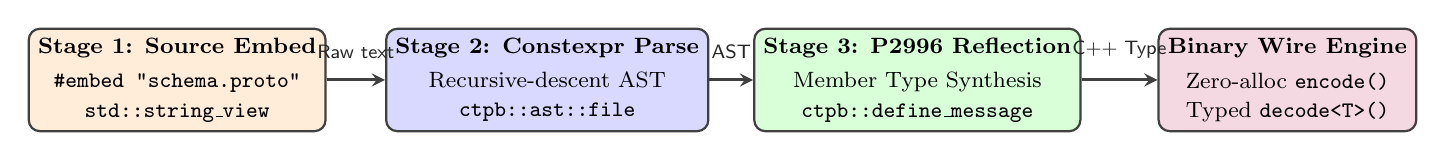
\begin{tikzpicture}[
    box/.style={
        rectangle, 
        draw=black!75, 
        thick, 
        minimum width=3.1cm, 
        minimum height=1.3cm, 
        align=center, 
        rounded corners=4pt, 
        font=\footnotesize
    },
    arrow/.style={
        ->, 
        >=stealth, 
        line width=1.1pt, 
        draw=black!75
    },
    labelnode/.style={
        midway, 
        above=4pt, 
        font=\scriptsize\sffamily, 
        text=black!85
    }
]
\node[box, fill=orange!15] (input) at (0,0) {\textbf{Stage 1: Source Embed}\\[3pt] \texttt{\#embed "schema.proto"}\\[1pt] \texttt{std::string\_view}};
\node[box, fill=blue!15] (parser) at (4.7,0) {\textbf{Stage 2: Constexpr Parse}\\[3pt] Recursive-descent AST\\[1pt] \texttt{ctpb::ast::file}};
\node[box, fill=green!15] (reflect) at (9.4,0) {\textbf{Stage 3: P2996 Reflection}\\[3pt] Member Type Synthesis\\[1pt] \texttt{ctpb::define\_message}};
\node[box, fill=purple!15] (wire) at (14.1,0) {\textbf{Binary Wire Engine}\\[3pt] Zero-alloc \texttt{encode()}\\[1pt] Typed \texttt{decode<T>()}};

\draw[arrow] (input.east) -- node[labelnode] {Raw text} (parser.west);
\draw[arrow] (parser.east) -- node[labelnode] {AST} (reflect.west);
\draw[arrow] (reflect.east) -- node[labelnode] {C++ Type} (wire.west);
\end{tikzpicture}
\caption{\texttt{ctpb} Three-Stage Compile-Time Reflection Pipeline.}
\label{fig:ctpb_pipeline}
\end{figure*}

\subsection{Pipeline Execution Stages}

\subsubsection{Stage 1: Source Embedding}
The user supplies the path to a \texttt{.proto} file as a template argument. In standard C++26, this is loaded using \texttt{\#embed} to yield a contiguous, immutable byte buffer. The buffer is mapped to a zero-copy \texttt{std::string\_view}.

\subsubsection{Stage 2: Constexpr Lexing and AST Construction}
The \texttt{ctpb::parser} class is instantiated inside a \texttt{consteval} context. It reads the string view and tokenizes the grammar on demand without backtracking. The parser outputs an immutable Abstract Syntax Tree representation (\texttt{ctpb::ast::file}) containing messages, fields, enums, oneofs, maps, reserved regions, and options.

\subsubsection{Stage 3: Reflection Splicing and Type Synthesis}
The function \texttt{define\_message} looks up the requested message entity in the parsed AST. Using P2996 static reflection (\texttt{define\_aggregate}), \texttt{ctpb} injects a struct definition with member variables matching each field and generates optimized \texttt{encode()} and \texttt{decode()} visitors directly into the AST of the active translation unit.

\subsection{User-Facing API Design}
The public API of \texttt{ctpb} provides an ergonomic, single-line interface for message generation and wire serialization:

\begin{lstlisting}[language=ModernC++, caption={User API in \texttt{ctpb}}]
#include <ctpb/ctpb.hpp>

// Compile-time schema synthesis
consteval { ctpb::define_message<"person.proto", "tutorial.Person">(); }
using Person = ctpb::message_t<"person.proto", "tutorial.Person">;

Person p{};
p.name = "Alex I. Tsvetanov";
p.id = 42;
p.email = "atsvetanov@tu-sofia.bg";

// Wire-format serialization
std::vector<std::byte> wire_data = ctpb::encode(p);

// Strongly-typed deserialization
auto decoded = ctpb::decode<Person>(wire_data);
if (decoded) {
    std::println("Decoded user: {}", decoded->name);
}
\end{lstlisting}
